\section{Results}
\label{sec:results}

Because Martel's approach defers selecting optimal options until the end of
equivalent expression discovery, we developed a method that could produce
exactly the same set of equivalent expressions from the traces computed by
Martel, and has the same time complexity, but we adopted it to generate a
Pareto frontier from the discovered expressions, instead of only error bounds.
This allows us to compare \marteltrace{}, \ie~our implementation of Martel's
method, against our methods \frontiertrace{} and \greedytrace{} discussed
in Section~\ref{sub:equivalent_expressions_analysis}. Fig.~\ref{fig:martel}
optimizes the expression ${(a + b)}^2$ using the three methods above, all
using depth limit $3$, and the input ranges are $a \in [5, 10]$ and $b \in [0,
0.001]$~\cite{martel07}. The IEEE754 single precision floating-point format
with rounding to nearest was used for the evaluation of accuracy and area
estimation. The scatter points represent different implementations of the
original expression that have been explored and analyzed, and the (overlapping)
lines denote the Pareto frontiers. In this example, our methods produce the
same Pareto frontier that Martel's method could discover, while having up to
50\% shorter run time. Because we consider an accuracy/area trade-off, we
find that we can not only have the most accurate implementation discovered by
Martel, but also an option that is only 0.0005\% less accurate, but uses 7\%
fewer LUTs.

We go beyond the optimization of a small expression, by generating results in
Fig~\ref{fig:multi_expr_32} to show that the same technique is applicable to
simultaneous optimization of multiple large expressions. The expressions $e_x$
and $e_y$, with input ranges $a \in [1, 2], b \in [10, 20], c \in [10, 200]$
are used as our example:
\begin{equation}
    \begin{aligned}
    e_x =& (a + a + b) \times (a + b + b) \times (b + b + c) \times {} \\
         & (b + c + c) \times (c + c + a) \times (c + a + a) \\
    e_y =& (1 + b + c) \times (a + 1 + c) \times (a + b + 1)
    \end{aligned}
\end{equation}

We generated and optimized RTL implementations of $e_x$ and $e_y$
simultaneously using \frontiertrace{} and \greedytrace{} with the depth limits
indicated by the numbers in the legend of Fig.~\ref{fig:multi_expr_32}. Note
that because the expressions evaluate to large values, the errors are also
relatively large. We set the depth limit to $2$ and found that \greedytrace{}
executes much faster than \frontiertrace{}, while discovering a subset of
the Pareto frontier of \frontiertrace{}. Also our methods are significantly
faster and more scalable than \marteltrace{}, because of its poor scalability
discussed earlier, our computer ran out of memory before we could produce
any results. If we normalize the time allowed for each method and compare
the performance, we found that \greedytrace{} with a depth limit $3$ takes
takes slightly less time than \frontiertrace{} with a depth limit $2$, but
produces a generally better Pareto frontier. The alternative implementations
of the original expression provided by the Pareto frontier of \greedytrace{}
can either reduce the LUTs used by approximately 10\% when accuracy is not
crucial, or can be about 10\% more accurate if resource is not our concern.
It also enables the ability to choose different trade-off options, such as
an implementation that is 7\% more accurate and uses 7\% fewer LUTs than the
original expression.

Furthermore, Fig.~\ref{fig:multi_expr_vary_width} varies the mantissa width of
the floating-point format, and presents the Pareto frontier of both $e_x$ and
$e_y$ together under optimization. Floating-point formats with mantissa widths
ranging from 10 to 112 bits were used to optimize and evaluate the expressions
for both accuracy and area usage. It turns out that some implementations
originally on the Pareto frontier of Fig.~\ref{fig:multi_expr_32} are no longer
desirable, as by varying the mantissa width, new implementations are both more
accurate and less resource demanding.

Besides the large example expressions above, Fig.~\ref{fig:taylor_sin} and
Fig.~\ref{fig:motzkin} are produced by optimizing expressions with real
applications under single precision. Fig.~\ref{fig:taylor_sin} shows the
optimization of the Taylor expansion of $\sin(x + y)$, where $x\in[-0.1, 0.1]$
and $y\in[0, 1]$, using \greedytrace{} with a depth limit $3$. The function
$\mathrm{taylor}(f, d)$ indicates the Taylor expansion of function $f(x, y)$ at
$x = y = 0$ with a maximum degree of $d$. For order 5 we reduced error by more
than 60\%. Fig.~\ref{fig:motzkin} illustrates the results obtained using the
depth limit $3$ with the Motzkin polynomial~\cite{demmel} $x^6 + y^4 z^2 + y^2
z^4 - 3 x^2 y^2 z^2$, which is known to be difficult to evaluate accurately,
especially using inputs $x\in[-0.99, 1]$, $y\in[1, 1.01]$, $z\in[-0.01, 0.01]$.

Finally, Fig.~\ref{fig:area} demonstrates the accuracy of the area estimation
used in our analysis. It compares the actual LUTs necessary with the estimated
number of LUTs using our semantics, by synthesizing more than 6000 equivalent
expressions derived from $a + b + c$, $(a + 1) \times (b + 1) \times (c + 1)$,
$e_x$, and $e_y$ using varying mantissa widths. The dotted line indicates exact
area estimation, a scatter points that is close to the line means the area
estimation for that particular implementation is accurate. The solid black line
represents the linear regression line of all scatter points. On average, our
area estimation is a 6.1\% over-approximation of the actual number of LUTs, and
the worst case over-approximation is 7.7\%.
\newcommand{\figsize}{0.6}
\begin{figure}[ht]
    \centering
    \includegraphics[scale=\figsize]{martel}
    \caption{Optimization of ${(a + b)}^2$}\label{fig:martel}
\end{figure}
\begin{figure}[ht]
    \centering
    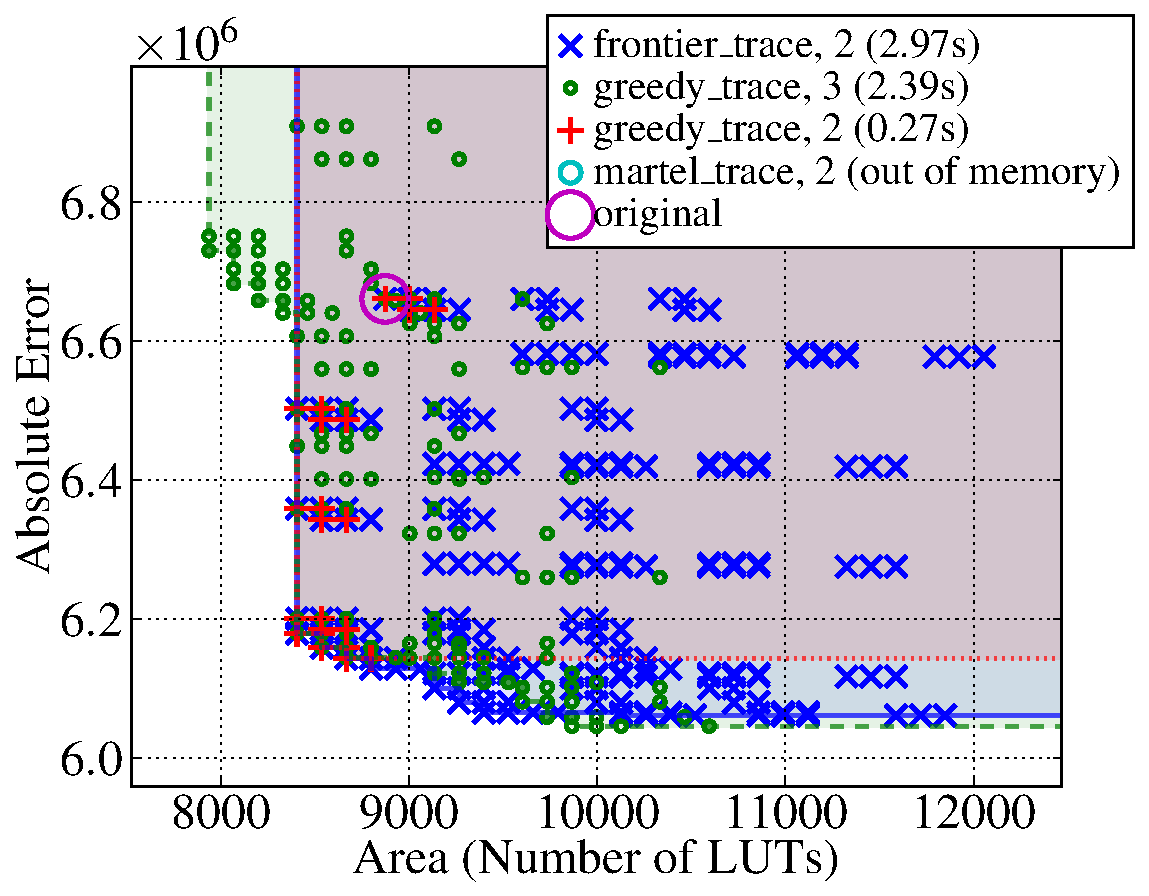
\includegraphics[scale=\figsize]{multi_expr_32}
    \caption{Simultaneous optimization of both $e_x$ and $e_y$}
    {}\label{fig:multi_expr_32}
\end{figure}
\begin{figure}[ht]
    \centering
    \includegraphics[scale=\figsize]{multi_expr_vary_width}
    \caption{Varying the mantissa width of Figure~\ref{fig:multi_expr_32}}
    {}\label{fig:multi_expr_vary_width}
\end{figure}
\begin{figure}[ht]
    \centering
    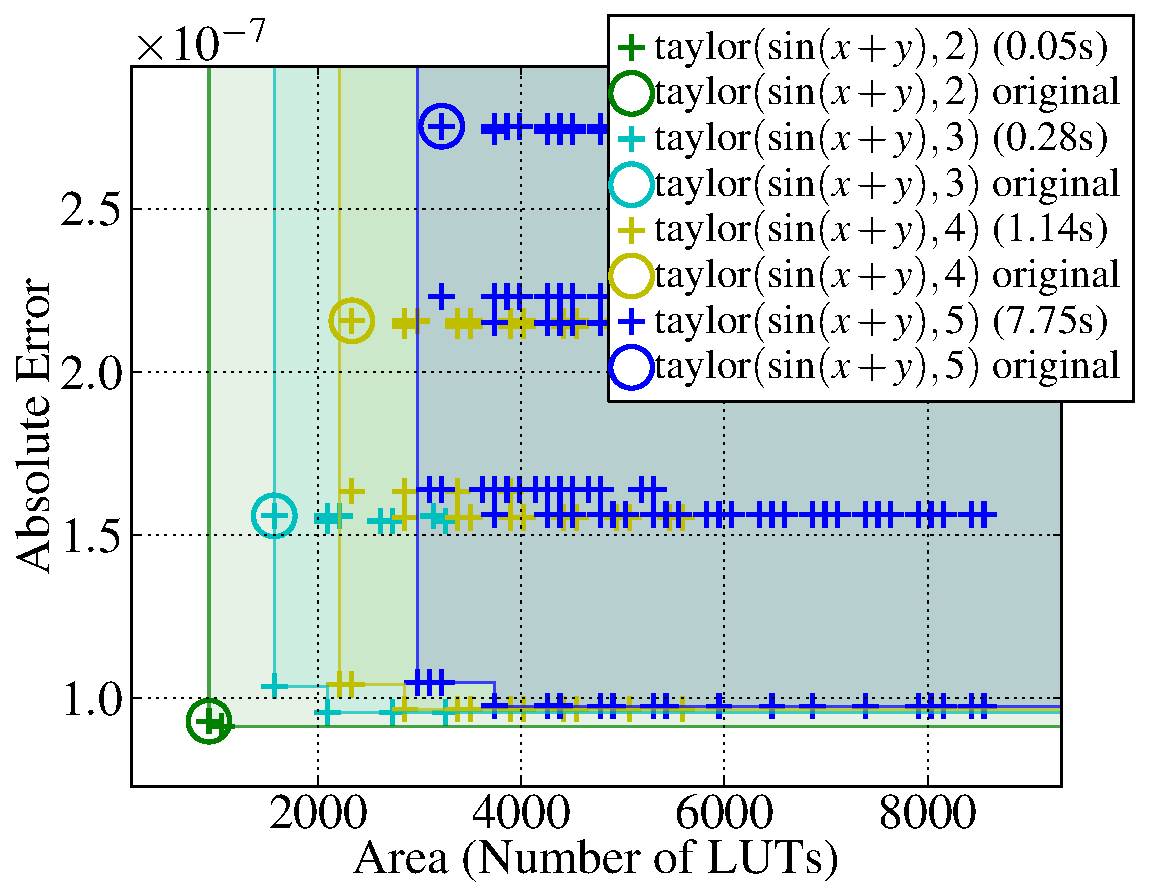
\includegraphics[scale=\figsize]{taylor_sin}
    \caption{The Taylor expansion of $\sin(x + y)$}
    {}\label{fig:taylor_sin}
\end{figure}
\begin{figure}[ht]
    \centering
    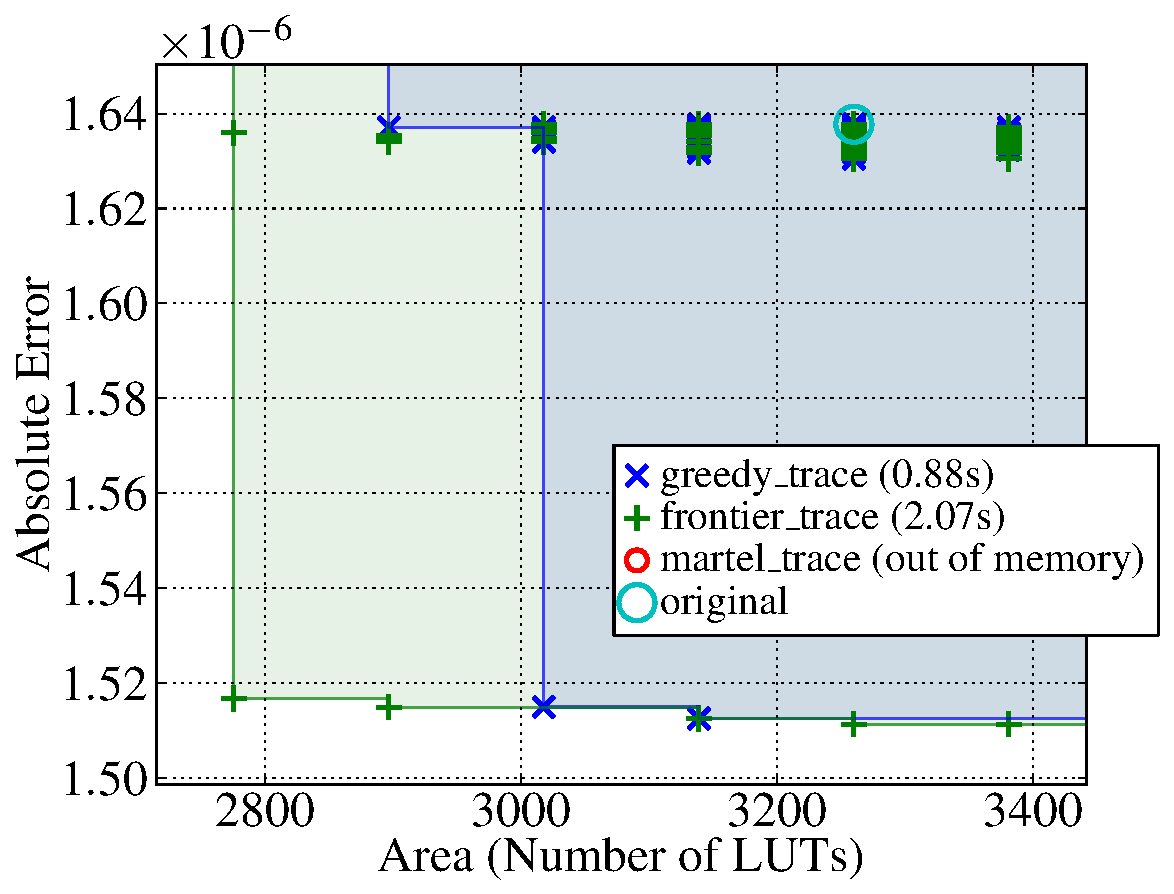
\includegraphics[scale=\figsize]{motzkin}
    \caption{The Motzkin polynomial $e_m$}\label{fig:motzkin}
\end{figure}
\begin{figure}[ht]
    \centering
    \includegraphics[scale=\figsize]{area}
    \caption{Accuracy of Area Estimation}\label{fig:area}
\end{figure}
